%%%%%%%%%%%%%%%%%%%%%%%%%%%%%%%%%%%%%%%%%%%%%%%%%%%%%%%%%%%
\subsection{Scattering Mechanisms}
%%%%%%%%%%%%%%%%%%%%%%%%%%%%%%%%%%%%%%%%%%%%%%%%%%%%%%%%%%%

Fresnel’s equations provide an explanation for light reflected and transmitted for ideal surfaces.  This is not the case with most man made and natural materials.  Therefore, more complex mechanisms must be considered when dealing with real world radiation scattering problems.  It has become popular in the field of remote sensing to denote the additional types of interactions as volume scattering and multiple scatter interaction.  Single scattering mechanisms are those governed solely by Fresnel’s equations.  The combination of these scattering mechanisms create the diffuse and specular components of reflection.

Single scattering mechanisms create a portion of reflectance known as specular reflectance.  They are often denoted as Type A photons in remote sensing models.  These interactions are highly polarized perpendicular to the plane of incidence as previously discussed. For perfectly smooth dielectrics, this is the dominate scattering mechanism.

Volume scattering occurs when light is absorbed by a material and is readmitted in all directions, including back towards the surface of the material.  They are denoted Type B photons.  Transmittance of this energy back into the first medium obeys the laws of Fresnel’s equations, although the indices of refraction are reversed.  This mechanism accounts for absorption and other higher level light matter interactions, not explained solely by Fresnel’s equations.

Multiple scattering occurs when either Type A or Type B photons interact with the material surface more than once when either being reflected or re transmitted out of the material.  These are denoted Type C photons \cite{schott}.  Figure 6 shows each type of interaction.
%
\begin{figure}[!htb]
    \begin{center}
        \makebox[\textwidth]{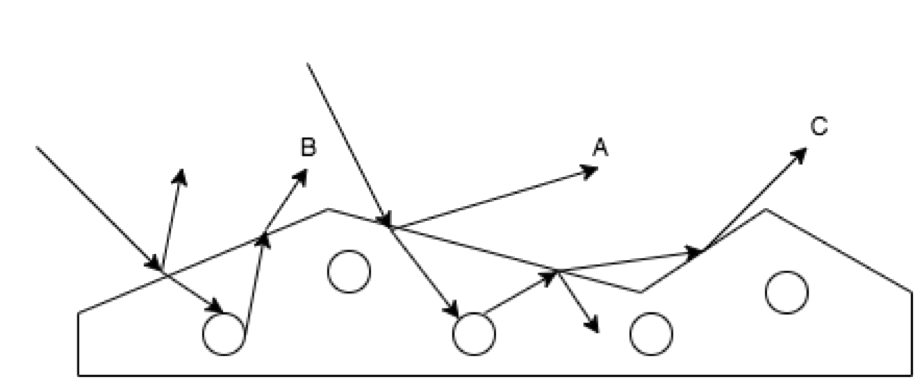
\includegraphics[scale=0.75]{/Sources/Background/Nature_of_Light/photon-interactions-wo.png}}
    \end{center}
    \caption{Various Types of Photon Interactions}
    \label{fig:scattering}
\end{figure}
%
In general type A photons create specular highlights from surfaces that are smooth.  Type B and C photons become more prevalent as a surface becomes rougher.  In most real world applications, surfaces are neither purely specular or purely diffuse.

Surfaces that are perfectly smooth dielectrics are often considered to be purely specular reflectors of light.  Incident energy is transmitted in an idealized single ray of light from the surface.  Specular reflectors are single scattering mechanisms and result in purely polarized light due to the governance of Fresnel’s equations and are denoted as type A photons.

In simple models, rough surfaces can be viewed as purely diffuse reflectors that scatter incident light equally in all directions.  Perfect diffuse surfaces are known as Lambertian surfaces.  It has been assumed that the diffuse portion of light is unpolarized due to random nature of internal reflections [\cite{specularclass}, \cite{grant}]. Bidirectional Reflectance Distribution Functions (BRDF) have been created to model the variety of surface interactions in order to handle the non ideal case of rough surfaces. (TODO in its simplest form rotational symmetry is assumed around the point of incidence and the equation becomes)
\begin{figure}[!htb]
    \begin{center}
        \makebox[\textwidth]{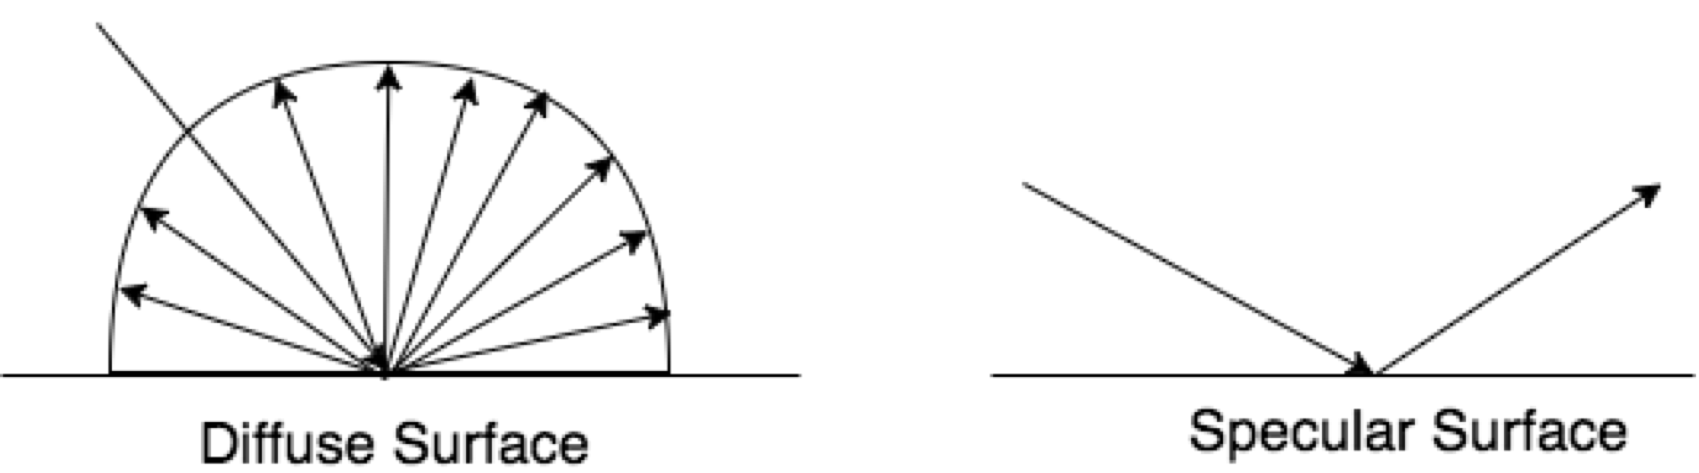
\includegraphics[scale=0.45]{/Sources/Background/Nature_of_Light/diffuse-specular.png}}
    \end{center}
    \caption{Diffuse and Specular Scattering}
    \label{fig:scattering}
\end{figure}

The notion of a surface being rough, smooth, fine or coarse come with the connotation of touch and the feeling of a materials' surface.  They are textures.
